\documentclass[a4paper,11pt]{article}
\setlength{\topmargin}{-.5in}
\setlength{\textheight}{9in}
\setlength{\oddsidemargin}{.125in}
\setlength{\textwidth}{6.25in}
\usepackage[pdftex]{graphicx}
\makeatletter
\renewcommand\paragraph{%
   \@startsection{paragraph}{4}{0mm}%
      {-\baselineskip}%
      {.5\baselineskip}%
      {\normalfont\normalsize\bfseries}}
\makeatother

\begin{document}

% The Title page
\begin{titlepage}
\begin{center}

\includegraphics[width=0.8\textwidth]{fig/eorlogo}\\[3cm]    
\textsc{\LARGE Description and usage of gainanim.py}\\[0.5cm]
\vfill
{\large 
\emph{Oscar Martinez} \\
University of Groningen \\ 
Kapteyn Astronomical Institute \\
Groningen \\
The Netherlands \\
\today}
\end{center}
\end{titlepage}

% INDEX
\tableofcontents
\newpage

\section {Introduction}

\textit{gainanim.py} (ans its LEDDB version) is intended to provide a way to generate a movie of all the stations gains for a LOFAR observation. The observation must have been calibrated and, hence, its SBs must contain valid instrument tables (filled with the GAIN records).

This script does not actually create a movie, it generates the \textit{pngs} and show the command to be run afterwards (\textit{ffmpeg} or \textit{mencoder}). 

\textit{gainanim.py} was originally written by Cyril Tasse (cyril.tasse@obspm.fr) and it has been modified and extended by Oscar Martinez.

\section {Options}

Use \textit{gainanim.py -h} to see all the options. In addition to the input and output options (more in next section), the main important option is to define whether the animation is in time or in frequency (by default is time). Moreover the user can choose the plotted complex coordinates, i.e Real-Imag or Ampl-Phase, the Jones matrix elements, the stations, the reference station, the y axis range, the times slots, the used frequency channels and the figure size.

It is worth mentioning that in the case of frequency animation, it is recommended to use a short number of time samples (for example with a large time step) given the resolution of the final station plots.

Optionally, the user can specify a delay file. If provided, this file must have a line for each station which gain phase we want to correct. When plotting the phase of the gains solution the following will be subtracted in each frequency sample: $2 \cdot pi \cdot freq[$MHz$] \cdot delay\_station$. An example of the content of a delay file is:

\begin{small}
\begin{verbatim}
RS106HBA 92.e-9
RS205HBA 88.e-9
RS208HBA 91.e-9
RS305HBA 94.e-9
RS306HBA 122.e-9 
RS307HBA 110.e-9
RS310HBA 99.e-9
RS406HBA 92.e-9
RS407HBA 97.e-9   
RS409HBA 87.e-9
RS503HBA 128.e-9
RS508HBA 171.e-9
RS509HBA 178.e-9
\end{verbatim}
\end{small}

When reading the gain solutions from the measurement sets (i.e. not using the LEDDB) the nodes containing the data are always used. However, when plotting with time animation, more nodes can be added and they will also be used in the generation of pictures. The user can also choose the number of workers used per node. How ever, depending on the case, these workers have different definition:
\begin{itemize}
\item In frequency animations, the specified workers are in charge of both gain reading and pictures generation.
\item In time animations, there are two type of workers: the read-workers and the plot-workers. Take into account that, for each node, we will create as many read-workers as number of SBs in the node. The latter is not configurable since we need to have all the SBs simultaneously accessed in order to combine the data. What the user specifies, in this case, is the number of workers used for the pictures generation (plot-workers). The recommended value is: \textit{numPlotWorkers = numProcessors - numSBsInNode}
\end{itemize}


The option port defines the TCP port used for the message passing between current machine and remote clients. There are other options related to the communication between the server and the clients (workers): \textit{chunkin} and \textit{chunkout}. They are only used in the case of time animations. 
\begin{itemize}
\item \textit{chunkin} is the chunk size of the gains (in time) requested by the server (in local machine) to the remote clients (read-workers). The higher the number the more RAM the local machine will need to combine the remote chunks. 
\item \textit{chunkout} is the chunk size of the combined gains (in time) send by the server (in local machine) to the remote nodes (plot-workers)
\end{itemize}

\section {Input and output}

In order to run the script the user must provide a GDS file. In time animations it is recommended that the given GDS file does not reference more than 40 SBs. Given the resolution of the final station plots, giving more SBs will not have a noticeable effect. Also, in this case all the solutions must be accessed simultaneously in order to combine them and this is considerably expensive (even though we facilitate this task by only sending small chunks of data).

The output folder will be filled with the logs, images and the information file. It is important to mention that this directory must be shared between the involved nodes (since remote clients will write the generated images in it).

\subsection {Using LEDDB stored gains}

It is also possible to use gains stored in the LEDDB. In this case you need to create a \textit{DiagFile} and use \textit{ExecuteLModule GAINAnimation} (instead of \textit{gainanim.py}). For the creation of the \textit{DiagFile} follow these steps:

\begin{itemize}
\item Use your favorite web browser to visit the LEDDB web. Use the same user name and password you use to access the LOFAR EoR cluster.
\item In the first tab (LDS) you can see the several observations. Pay attention to \textit{hasGain} column. Select an observation with \textit{hasGain = True}.
\item Go to the second tab (LDSB) and select a beam (pay also attention that the selected beam also has \textit{hasGain = True}.
\item Go to the third tab (LDSBP). Here you can see several versions of the data for the selected observation-beam. Select a row (version) also paying attention to \textit{hasGain} column.
\item Go to the fourth tab (MS). You will see all the SBs for that observation-beam-version. You can use \textit{Filter} to select only some SBs. For example, in the case of time animation you could add a Filter for: 

 \textit{sbIndex = 0, 10, 20, 30, 40, 50, 60, 70, 80, 90, 100, 110, 120, 130, 140, 150, 160, 170, 180, 190, 200, 210, 220, 230, 240, 250, 260, 270, 280, 290, 300, 310, 320, 330, 340, 350, 360, 370}.
\item After you are done with the filtering in LDSBP, select all the rows and go to GAIN tab.
\item Select all the rows (you can use the click box in the header) and click in \textit{Save DiagFile}.
\end{itemize}

Now you are ready to run the \textit{ExecuteLModule GAINAnimation} by providing the \textit{DigFile} as input (instead of the GDS file). You also need to specify the nodes that you will use. The rest of options are exactly the same than in \textit{gainanim.py}.

\section { Logging and \textit{INFO} file }

Once you are running the script, you can check the progress of the server in the standard output. The several remote clients log their progress in files in the output directory. Check the \textit{.log} files.

In addition to the log files and the images, this script also creates a \textit{INFO} file which contains a summary of the used options. This intends to provide enough information for a possible future re-generation of the movie.

\section { Tutorial}

\subsection {Time animation}

We want to create a animation (in time) from some calibrated data . As we previously mentioned, in this case it is not advisable to use all the SBs (because we need to simultaneously read them in order to combine them and split them in time). We use the following 38 SBs: 0,10,20,30..380 (obviously, any other set of SBs is also possible)

First we need to create the 38 VDS files. Second, we create a single GDS file containing referencing the 38 SBs. We run the script with the following command:

\begin{small}
\begin{verbatim}
python gainanim.py -i 38SBs.gds -o 38SBs_time_animation -n node011-074 -w 15
\end{verbatim}
\end{small}

This will create images (as many as time samples) using the 38 SBs pointed in the GDS file. It will use the folder \textit{38SBs\_time\_animation} (it is created if it does not exist) as output directory for the logs, images and information file. We use the option \textit{-n} to specify that for the generation of images we want to use \textit{node011-node074}. Some of these nodes would have been anyway used since they contain data (and nodes containing data are always used). We also use \textit{-w 15}, this means that each remote client will create 15 plot-workers. We do this because, in this case, the nodes contain 1 SB and hence we will require an additional read-worker to load the gain solutions. In this way we guarantee we do not use more than 16 processes in any node. Be specially careful if your GDS refers to nodes with several SBs. Remember that for each SB in a node we need to create a read-worker in the node. Size the \textit{numworkers} option accordingly in order to avoid saturating the nodes. 

For the rest of options we use their default value: obviously the \textit{xaxis} option is set to frequency (which means that the animation is in time), only \textit{0,3} (XX and YY) are used from the Jones matrix, all stations are used, the reference station is the first one, we use polar coordinates, all times samples are used, only first channel is used, etc.

After the script is finished the last lines will show which command you need to run to create the animation (two options are given: \textit{mencoder} and \textit{ffmpeg}). For example, for \textit{ffmpeg}:

\begin{small}
\begin{verbatim}
ffmpeg -r 20 -i 38SBs_time_animation/img%06d.png -vcodec mpeg4 -b:v 4620000 -y animation.mp4
\end{verbatim}
\end{small}

A snapshot of the generated movie is shown in \ref{fig:time}.

\begin{figure}[h]
  \centering
  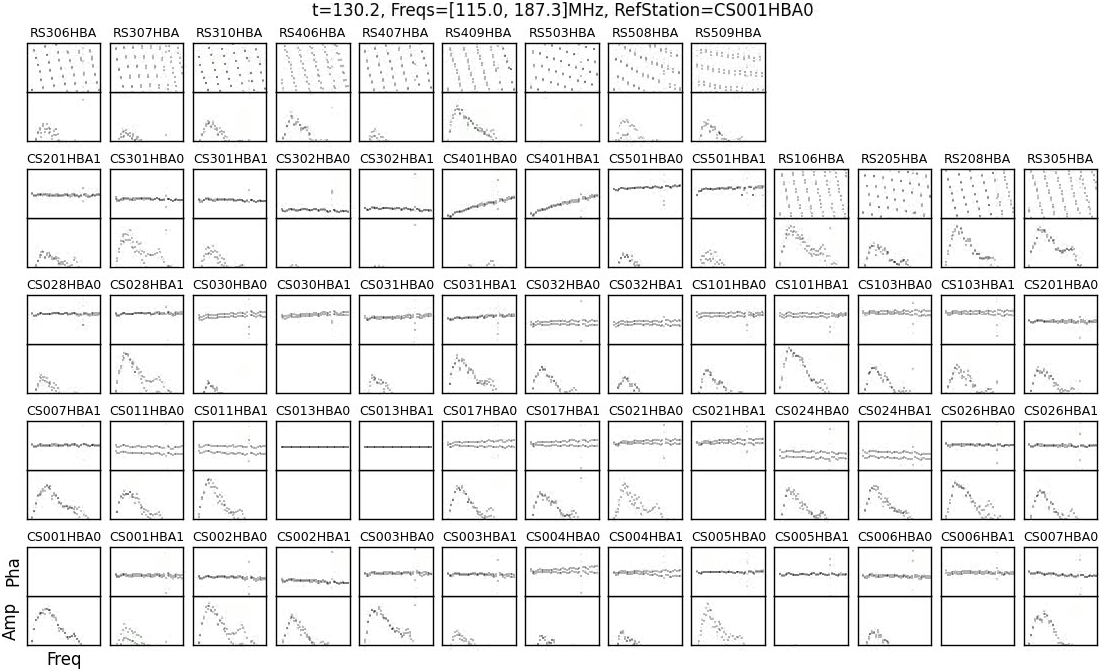
\includegraphics[scale=0.52]{fig/time} 
  \caption{Snapshot of a time animation}
  \label{fig:time}
\end{figure}

\subsection {Frequency animation}

We want to create a animation (in frequency) from some calibrated data. In this case we can use all the SBs since the processing is not so intensive as animating in time (because we do not need to read all SBs simultaneously). In fact, we want as many frequencies as possible in order to have a more frames in the animation. As in the previous case, we need to create the VDS files and a single GDS file. We run the script with the following command:

\begin{small}
\begin{verbatim}
python gainanim.py -i 380SBs.gds -o 380SBs_freq_animation -x time -t 1000,2000,50
\end{verbatim}
\end{small}

This will create images (as many as frequency samples, in this case $380 \cdot numChan$) using the 380 SBs pointed in the GDS file. It will use the folder \textit{380SBs\_freq\_animation} (it is created if it does not exist) as output directory for the logs, images and information file. In this case, we have to specify the \textit{xaxis} (\textit{-x time}) since it is not the default one. We also specify \textit{-t 1000,2000,50}, this will use only the time samples from 1000 to 2000 in steps of 50. 

Fro the rest of options we use their default value: only \textit{0,3} (XX and YY) are used from the Jones matrix, all stations are used, the reference station is the first one, we sue polar coordinates, only first channel is used, etc. 

Note that in this case we also use the default number of workers. In frequency animations each worker is already in charge of reading and plotting so we do not require extra read-workers.

After the script is finished the last lines will show which command you need to run to create the animation (two options are given: \textit{mencoder} and \textit{ffmpeg}). For example, for \textit{ffmpeg}:

\begin{small}
\begin{verbatim}
ffmpeg -r 4 -i 38SBs_freq_animation/img%06d.png -vcodec mpeg4 -b:v 4620000 -y animation.mp4
\end{verbatim}
\end{small}

A snapshot of the generated movie is shown in \ref{fig:freq}.

\begin{figure}[h]
  \centering
  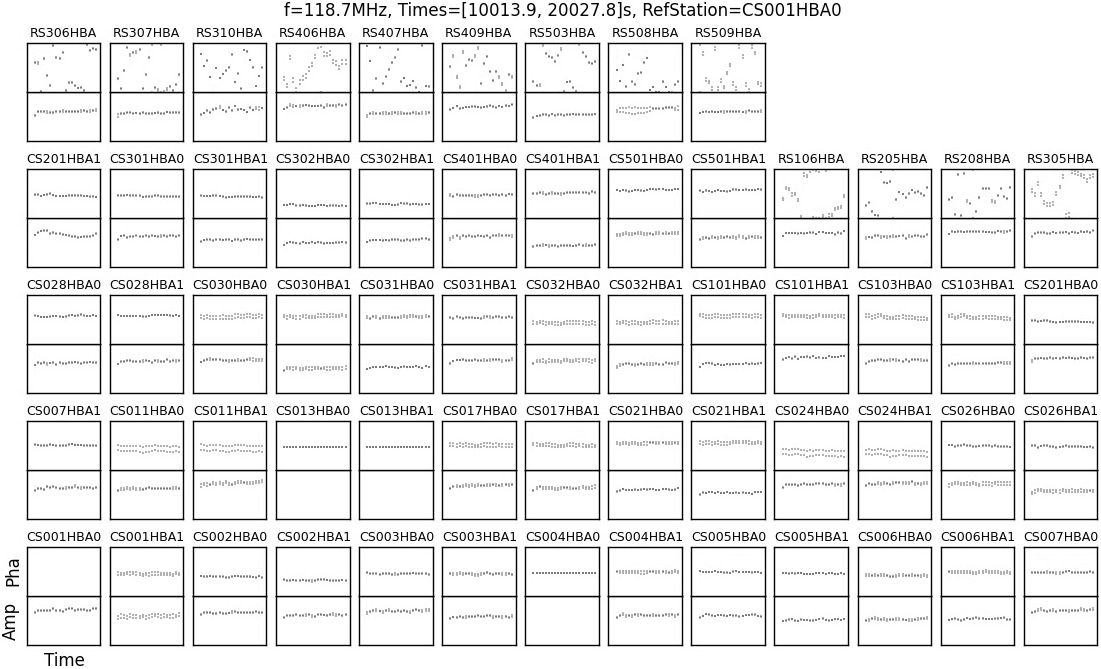
\includegraphics[scale=0.52]{fig/freq} 
  \caption{Snapshot of a frequency animation}
  \label{fig:freq}
\end{figure}

\end{document}